\chapter{Five Skills Every Young Man Should Know}

This chapter is built from an interview rather than a blackboard lecture, but the talk still has a precise internal structure. The host asks Nico Lagan for a compact curriculum for young men, especially for those who have grown up without strong male guidance. What follows is a five-step sequence: first bodily competence, then action under fear, then guidance, then provision, then self-mastery, and finally faith. We will keep close to the order of the transcript, and where the lecture naturally condenses itself into a formal pattern, we will write that pattern down.

No validated board images survive from this lecture, so every formula below is a note-taking reconstruction of the spoken logic rather than a literal transcription from a board. The point is not to force mathematics into the interview, but to preserve its structure with as much rigor as the source permits.

\section{Introduction and the Ordered Curriculum}

The lecture begins with an explicit promise: five skills that every young man should master in today's world. The host's personal framing matters. He says that he grew up without a male figure, and this turns the list into a repair manual rather than a vague motivational exercise. We are not being offered a pile of virtues. We are being given an ordered curriculum.

\begin{definition}
We denote the lecture's ordered five-skill sequence by
\begin{equation}
\Sigma=(\sigma_1,\sigma_2,\sigma_3,\sigma_4,\sigma_5)
=(\mathrm{Protection},\mathrm{Courage},\mathrm{Provision},\mathrm{Temperance},\mathrm{Faith}).
\end{equation}
\end{definition}

The order matters. Protection comes first because the lecture begins with the question of what a man must be able to do. Courage follows because the mere possession of tools does not yet produce action. Provision widens the frame from self to family. Temperance asks how a man governs himself. Faith is saved for the end because it marks the limit of direct control.

\begin{remark}
The symbols in this chapter are not part of the original spoken language of the lecture. They are a compact way of preserving the progression and the internal contrasts that the speaker uses.
\end{remark}

\begin{figure}[h]
\centering
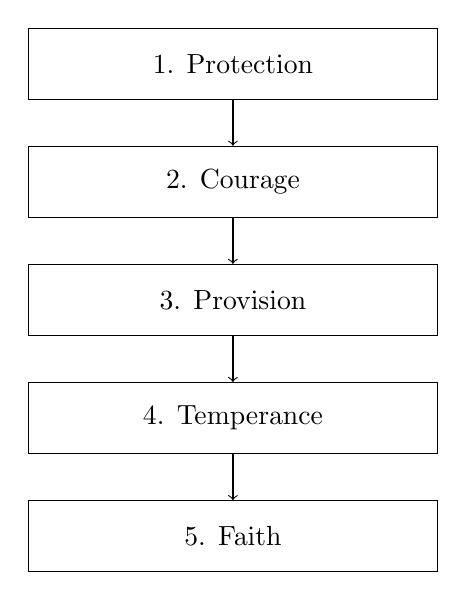
\begin{tikzpicture}
\node[draw, align=center, minimum width=5.2cm, minimum height=0.9cm] (s1) at (0,0) {1. Protection};
\node[draw, align=center, minimum width=5.2cm, minimum height=0.9cm] (s2) at (0,-1.5) {2. Courage};
\node[draw, align=center, minimum width=5.2cm, minimum height=0.9cm] (s3) at (0,-3.0) {3. Provision};
\node[draw, align=center, minimum width=5.2cm, minimum height=0.9cm] (s4) at (0,-4.5) {4. Temperance};
\node[draw, align=center, minimum width=5.2cm, minimum height=0.9cm] (s5) at (0,-6.0) {5. Faith};

\draw[->] (s1.south) -- (s2.north);
\draw[->] (s2.south) -- (s3.north);
\draw[->] (s3.south) -- (s4.north);
\draw[->] (s4.south) -- (s5.north);
\end{tikzpicture}
\caption{A transcript-based map of the lecture's vertical sequence. The motion is from bodily competence to action, then to responsibility, self-mastery, and finally belief.}
\end{figure}

\section{Protection: Self-Defense and Physical Maintenance}

The first skill is protection. The lecture does not define this in sentimental terms. A protector must know how to defend himself, and he must also be physically fit. Nico folds the two together: martial arts on one side, bodily maintenance on the other.

There is a useful metaphor here. The body is treated as a machine. One does not put bad gas in a car and then expect it to run well; by analogy, one should not sabotage the body and then expect it to function under pressure. The transcript does not turn this into a physiology model, so we should resist inventing one. But the analogy does serve a structural purpose: it links protection to maintenance. Self-defense is not just a technique. It presupposes care of the instrument that must carry it out.

\subsection{Question \& Answer}

\paragraph{Question.} If martial arts matter, what should a beginner learn first?

\paragraph{Answer.} Nico's answer is Muay Thai. He is careful not to dismiss boxing. He explicitly says that boxing is not the easiest martial art, but that it is the simplest in the narrow sense that it uses only the fists. His preference for Muay Thai is then justified operationally: there are more tools available, and there is more control at close range.

We can write the comparison as a very compact transcript-backed tool-set contrast:
\begin{align}
\mathcal{B}_{\mathrm{tools}} &= \{\mathrm{fists}\},\\
\mathcal{M}_{\mathrm{tools}} &= \{\mathrm{fists},\mathrm{elbows},\mathrm{knees},\mathrm{kicks},\mathrm{close\ control}\}.
\end{align}
Within the lecture's restricted comparison, we therefore have
\begin{equation}
\mathcal{B}_{\mathrm{tools}} \subset \mathcal{M}_{\mathrm{tools}}.
\end{equation}

The point is practical rather than abstract. Boxing relies on the hand against a hard target. Nico adds the concrete warning that in a real fight the hand can break against a skull. Muay Thai, by contrast, offers additional striking surfaces and close-range management.

\begin{table}[h]
\centering
\begin{tabular}{|p{0.18\linewidth}|p{0.28\linewidth}|p{0.28\linewidth}|}
\hline
Aspect & Boxing & Muay Thai \\
\hline
Tools emphasized in the lecture & Fists only & Fists, elbows, knees, kicks \\
\hline
Practical range & Lecture stresses punching & Lecture adds close control \\
\hline
Real-fight concern & Hand may break against a skull & More striking options are available \\
\hline
\end{tabular}
\caption{The lecture's practical comparison. Boxing is called simpler, not easier. Muay Thai is preferred because it enlarges the usable set of tools.}
\end{table}

This closes the first skill in the way the lecture itself closes it: not with a slogan, but with a concrete recommendation.

\section{Courage: Preparation Must Cross into Action}

The second skill is courage. The transition is explicit in the lecture: the first point was self-defense; now we move to courage. This is the first major sharpening of the argument. Protection gives us capacity. Courage asks whether capacity ever becomes action.

Nico's central claim is nearly aphoristic: one may have the best plan on the planet and be as mentally prepared as possible, but without courage none of it moves. We can formalize the claim schematically as
\begin{align}
\mathrm{Preparation}\land \neg \mathrm{Courage} &\Rightarrow \mathrm{No\ decisive\ action},\\
\mathrm{Preparation}\land \mathrm{Courage} &\Rightarrow \mathrm{Action}\to \mathrm{Confidence}.
\end{align}

\begin{proposition}
Within the logic of the lecture, preparation is necessary but not sufficient. Courage is the enabling term that converts preparation into action.
\end{proposition}

\begin{proof}
The lecture's argument is direct. People become stuck in what Nico calls preparation mode because they are afraid to take the first step. Fear is therefore not a lack of planning, but an obstruction that planning alone does not remove. The moment courage is supplied, the prepared plan becomes executable. Once executed, repeated action produces confidence, which in turn strengthens future action.
\end{proof}

The important point is that courage is not presented as the absence of fear. The lecture never says that fear disappears. It says that fear ceases to veto action.

\subsection{Question \& Answer}

\paragraph{Question.} Can courage be improved, or is it simply natural?

\paragraph{Answer.} Nico answers that it can be improved, and he answers by example rather than abstraction. He describes himself as bullied and scared when he was young. Then martial arts enter the story, first as self-defense and then as a school of confidence. He goes further and says that he stepped into a ring for roughly a dozen amateur fights, terrified each time, in order to prove to himself that he could face an opponent and face fear.

This creates a natural sequence:
\begin{enumerate}
\item Fear is present.
\item Training increases capability.
\item Capability makes action available.
\item Repeated action under fear produces confidence.
\item Confidence does not abolish fear, but it prevents fear from deciding the outcome.
\end{enumerate}

We can compress the lecture's logic into the following chain:
\begin{equation}
\mathrm{Fear}\to \mathrm{Training}\to \mathrm{Action\ under\ fear}\to \mathrm{Confidence}.
\end{equation}

One should read this as a summary of the argument, not as a mechanical law. The lecture is preserving a lived pattern: courage can be cultivated by repeated contact with difficult situations.

\section{Mentorship and the Recovery of Guidance}

After a short interruption, the lecture resumes with a new question: what should a young man do if he has no father figure? The answer begins generously. We are told that we live in a fortunate age because online material, videos, and public examples are widely available. But the answer does not stop there. Nico immediately adds a qualification: that is not enough.

The insufficiency matters. Online images can be a front. Social media can display a persona without transmitting character. The lecture therefore returns to martial arts, but now in a third role. Martial arts were first the school of self-defense, then the school of courage, and now they become the institutional setting in which coaches function as mentors.

This is a small but important bridge in the architecture of the talk. The lecture does not move from courage to provision by accident. It inserts the question of guidance, and the answer is that real discipline is usually carried by people, institutions, and repeated contact. Coaches matter because they embody standards, not merely advice.

\section{Provision Before Family}

The third skill is provision. Here the lecture widens from the self to the household. Nico's first move is temporal: one should not wait until a family appears in order to become a provider. The work begins earlier.

That temporal structure can be written schematically as
\begin{equation}
t_{\mathrm{prov\_start}} < t_{\mathrm{family\_formation}}.
\end{equation}

The lecture then turns normative. Nico says that a man must bring money into the relationship and describes this as what a man brings ``to the equation.'' We should be careful here. The transcript is garbled in one short passage, and the claim itself is clearly the speaker's norm rather than an objective theorem of household economics. Still, the structure of the argument is clear enough to preserve:
\begin{enumerate}
\item Provision is a duty, not an afterthought.
\item It must begin before the family exists.
\item Its purpose is to make care of the family possible.
\end{enumerate}

\begin{remark}
This section should remain close to the lecture's wording and should not be inflated into a formal model of gender economics. The chapter should preserve the claim as Nico's stated view about responsibility in a relationship.
\end{remark}

The transition out of this section is again explicit in the transcript. Once external responsibility has been named, the lecture asks what kind of inner discipline is needed to carry it. That is the door into temperance.

\section{Temperance: The Control Set}

The fourth skill is temperance, and Nico glosses it in a stoic register as self-mastery. This is the part of the lecture with the clearest compact formal spine. We are told that one controls only three things:
\begin{equation}
\mathcal{K}=\{\mathrm{emotions},\mathrm{actions},\mathrm{reactions}\}.
\end{equation}
Everything else falls outside that set:
\begin{equation}
\mathcal{X}_{\mathrm{external}}=\mathrm{Life}\setminus \mathcal{K}.
\end{equation}

This is a sharp partition. The lecture is not saying that emotions do not exist, or that action is easy. It is saying that moral labor should be directed to the terms inside \(\mathcal{K}\), because the rest of life does not submit to our command.

\paragraph{Worked example: the traffic incident.}
Nico gives a simple case. Suppose another driver cuts us off in traffic. The external event itself is not ours to govern. What remains ours is what we do next.

Let \(e\) denote the event of being cut off, and let \(r\) denote our reaction. Then
\begin{align}
e &\in \mathcal{X}_{\mathrm{external}},\\
r &\in \mathcal{K}.
\end{align}
If the reaction is impulsive, the lecture gives a clear escalation chain:
\begin{equation}
e \to r_{\mathrm{impulsive}} \to \mathrm{Escalation} \to \mathrm{Bad\ outcome}.
\end{equation}
If instead the reaction is restrained, the chain is cut:
\begin{equation}
e \to r_{\mathrm{restrained}} \to \mathrm{No\ escalation}.
\end{equation}

The point of the example is not merely etiquette. It is an explicit update in attention. The event \(e\) lies outside \(\mathcal{K}\), so rational effort returns from the external trigger to the internal response. The lecture's short practical summary is: it doesn't matter. That sentence is not resignation. It is a rule for refusing useless escalation.

\section{Faith and the Limit of Direct Control}

The fifth and final skill is faith. The lecture now turns to a different register. Up to this point we have been talking about skills that can be trained, practices that can be repeated, and structures that can be disciplined. Faith is placed in the sequence precisely because it is unlike the others.

\subsection{Question \& Answer}

\paragraph{Question.} Why does faith belong on the list at all, and why does it come last?

\paragraph{Answer.} Nico says that faith matters because it is the only one of the five skills over which one does not have the same kind of direct control. One either believes or one does not. He then broadens the claim inductively: if we read enough biographies of great men, we repeatedly find belief in something larger than the self.

We can summarize the distinction in a compact way:
\begin{equation}
\{\sigma_1,\sigma_2,\sigma_3,\sigma_4\}\subseteq \mathcal{T}_{\mathrm{trainable}},
\qquad
\sigma_5\notin \mathcal{D}_{\mathrm{direct\ control}}.
\end{equation}

This is not a metaphysical proof. It is a classification inside the lecture. Protection, courage, provision, and temperance are framed as disciplines that can be practiced. Faith is framed as an orientation toward a larger force, whether one calls that force God, the universe, or nature. It comes last because it marks the boundary of the domain that sheer training can master.

\section{Summary}

The lecture gives us a compact, ordered map rather than an essay of disconnected virtues. First we learn protection, because a man must be able to defend himself and care for the instrument of action. Then we add courage, because preparation without action remains inert. Mentorship enters as the social structure that carries training into character. Provision widens responsibility outward toward family. Temperance supplies the stoic control map, reducing our governable domain to emotions, actions, and reactions. Faith then stands at the far edge of the sequence, as the one element the speaker treats as indispensable yet not directly trainable.

Taken together, the chapter is best read as an interview-derived curriculum in responsibility under pressure. Its formulas are schematic, but the structure is real, and that structure is what the notes should preserve.